\chapter{Condiciones de diseño}

\minitoc
Las condiciones de proyecto establecidas determinan el contenido de calor del aire, tanto del interior como del exterior, y afectan directamente a la capacidad del equipo de acondicionamiento. En este capítulo se explicarán los tipos de cargas que pueden existir en un sistema y cómo calcularlas.


Se entiende como \gls{carga-refrigeracion}, a la cantidad de calor que hay que extraer en verano o incorporar en invierno para producir y mantener en el espacio acondicionado ciertas temperatura y humedad prefijadas. Pueden clasificarse en dos partes fundamentales, según la época del año:
\begin{itemize}
	\item En verano, cargas de refrigeración.
	\item En invierno, cargas de calefacción.
\end{itemize}

Las unidades que usualmente se utilizan en el diseño de los equipos de refrigeración, son los siguientes:
\begin{itemize}
	\item \textbf{Frigoría/hora:} capacidad de un sistema de refrigeración para absorber calor en una hora. Equivale a $1.163$ W/h.
	\item \textbf{Tonelada de refrigeración.} Se considera igual a $3000$ frig/h.
	\item \textbf{KW:} es una unidad de potencia, que es igual a $860$ frig/h.  
\end{itemize}

\section{Condiciones de proyecto}

\ver{estaría bueno comentar cómo se toman los valores en la ashrae, ya que lo mencioné.}

\subsection{Condiciones externas}

Los valores de temperaturas de bulbo seco y húmedo, y la humedad relativa del exterior se obtienen de la base de datos de ASHRAE Climatic Design Conditions \parencite{ashrae2025conditions} según la localización. Las tablas muestran información para el cálculo de la carga de refrigeración (Annual Cooling) y calefacción (Annual Heating), y las condiciones climáticas según el mes (Monthly Climatic).

Como indica \textcite{carrier2009}, las temperaturas exteriores se establecen con base en distintos niveles \emph{percentiles}. El nivel percentil indica el porcentaje de horas durante los meses del período considerado en los que las temperaturas indicadas son superiores o iguales a las máximas dadas. 

\subsubsection{Condiciones en verano}

Las temperaturas a considerar serán las correspondientes a los percentiles $0.4\%$, $1\%$ y $2\%$. En la \autoref{fig:ashrae-conditions} se muestran los datos obtenidos de \textcite{ashrae2025conditions} de las condiciones para la carga de calefacción en Reconquista.

\begin{figure}
	\centering\caption{Condiciones climáticas anuales para cálculo de carga de refrigeración, deshumidificación y entalpía. \emph{Fuente: ASHRAE Climatic Design Conditions.}}
	\label{fig:ashrae-conditions}
	%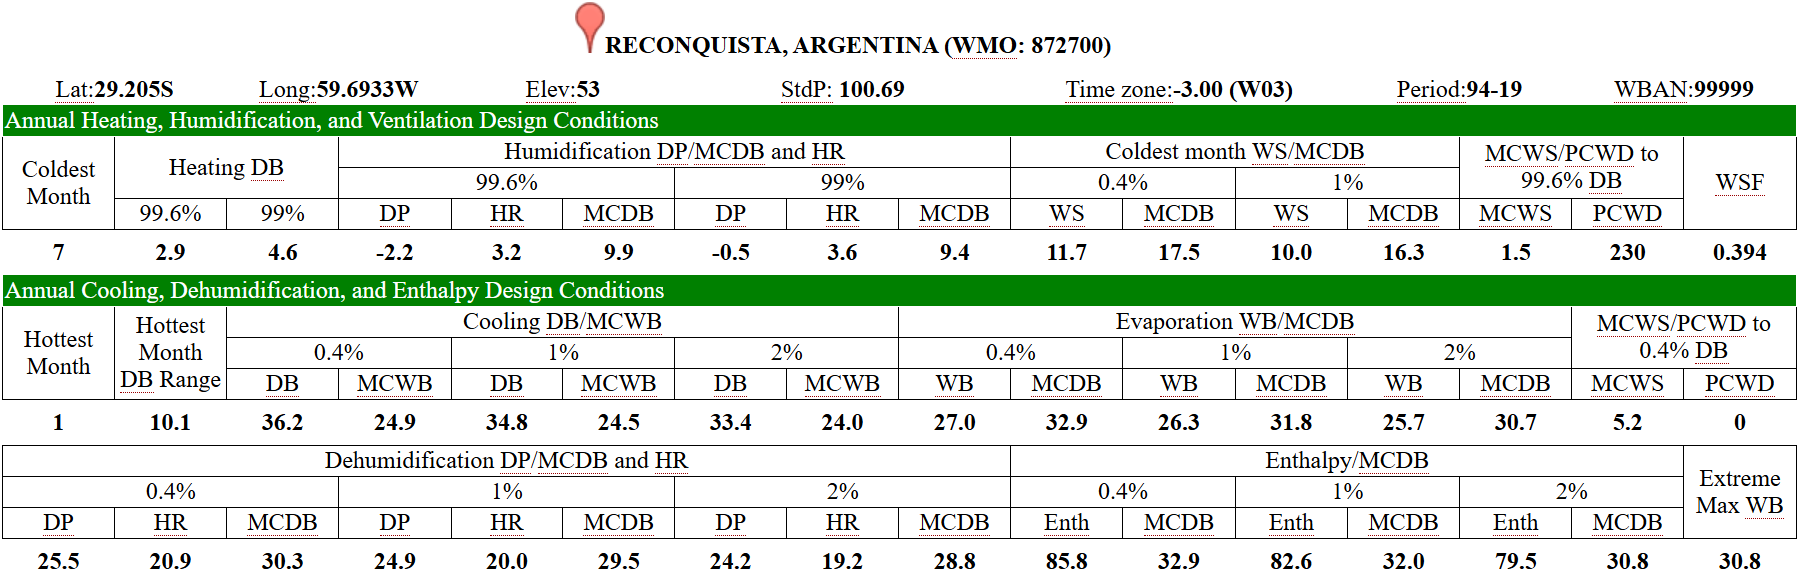
\includegraphics[width=\linewidth]{ashrae-conditions}
	
\end{figure}

El percentil del $0.4\%$ indica que, considerando esas temperaturas de diseño, las condiciones exteriores superarán dicho valor durante aproximadamente el $0.4\%$ del total de horas de ese mes. Por lo tanto, el sistema podría quedar subdimensionado durante ese tiempo.

Según \textcite{carrier2009}, se considera
\begin{itemize}
	\item nivel percentil de $1\%$ para hospitales, clínicas, sala de ordenadores y cualquier otro espacio que el diseñador crea necesario tener esa cobertura,
	\item nivel percentil de $2.5\%$ para edificios de especial consideración,
	\item nivel percentil de $5\%$ como norma general.
\end{itemize}

\subsubsection{Condiciones en invierno}

Según \citeauthor{ashrae2025conditions}, las temperaturas a considerar serán las correspondientes a los percentiles $99.6\%$ y $99\%$. En la \autoref{fig:ashrae-conditions} se muestra la tabla obtenida de \textcite{ashrae2025conditions} de las condiciones para la carga de calefacción en Reconquista.

\subsubsection{Corrección de temperatura}

En invierno, la temperatura exterior puede considerarse prácticamente constante durante el día, sin errores significativos. En verano, en cambio, las variaciones son mayores, y según la aplicación, se usan tablas de corrección de temperatura y humedad para evitar sobredimensionar el sistema. Por ejemplo, si bien los datos disponibles de temperatura máxima son a las 15 horas, en establecimientos con actividad nocturna  esa condición no se alcanza por el horario tardío en el que operan, por lo que se ajusta a una temperatura menor.

La \autoref{fig:correccion} muestra correcciones de temperaturas exteriores y humedades relativas para distintas horas del día.

\begin{figure}
	\centering
	\caption{Correcciones de temperaturas exteriores y humedades relativas para otras horas del día en Argentina. \emph{Fuente: \textcite[Cuadro 8-I]{quadri2020}.}}
	\label{fig:correccion}
	%%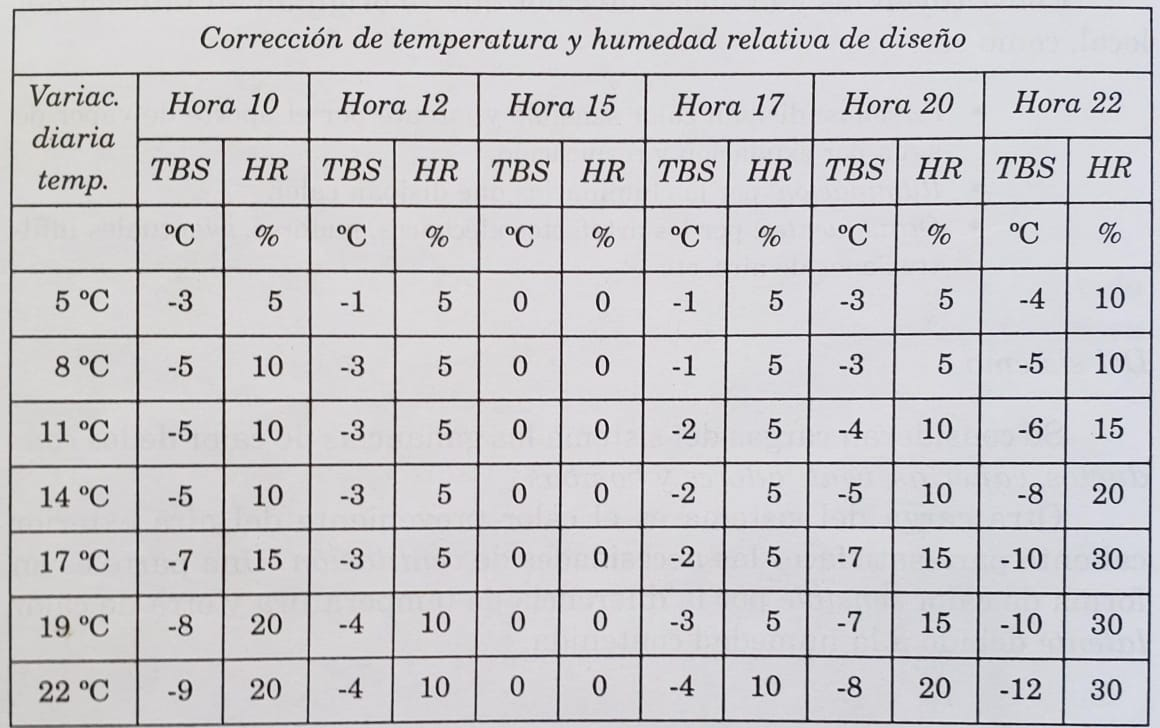
\includegraphics[width=0.7\linewidth]{correccion}
\end{figure}

\subsection{Condiciones internas}

\subsubsection{Verano}
Estas condiciones son \parencite{carrier2009}: una temperatura operativa comprendida entre 23 y 25°C, y una humedad relativa entre el 45 y 60\%.

\subsubsection{Invierno}
Estas condiciones son: una temperatura entre 21 y 23°C, y una humedad relativa comprendida entre el 40 y 50\%.

\subsubsection{Condiciones internas para la industria}
La Tabla 5 del manual de \citeauthor[pág. I-12]{carrier2009}, presenta las temperaturas y humedades relativas utilizadas en distintas aplicaciones. Es importante destacar que algunas de estas condiciones fueron establecidas principalmente para mejorar el confort del personal que trabaja en el área, más que por su efecto directo sobre el producto.